\documentclass{article}
%% Fix so sections are manually numbered
\setcounter{secnumdepth}{0}
%% Stop text from indenting
\setlength\parindent{0pt}

%% Graphics are stored in the graphics path
\usepackage{graphicx}
\graphicspath{ {./Latex/graphics/} }

%% Making hyperlinks in the table of contents
\usepackage{hyperref}
\hypersetup{
    colorlinks,
    citecolor=black,
    filecolor=black,
    linkcolor=blue,
    urlcolor=black
}

\title{Jammertest Testplan}
\author{Jammertest Consortium}
\date{ }

\begin{document}
\maketitle

\includegraphics[scale=0.1]{NPRA.png}

\tableofcontents

\section{Introduction}
Jammertest is a government initiative to create a tasted for industry, academia and other authorities in ensure robust use of Global Navigation Satellite Systems (GNSS). A testbed is a controlled environment where activities that are not allowed under normal conditions can be carried out safely under control of the authorities. Jammertest is a specific type of testbed where five Norwegian authorities have come together and creates an environment where GNSS jamming, spoofing and meaconing is present under controlled conditions in a real world outdoor environment.

This test plan describes all planned test cases that can be executed at the Jammertest event at Bleik, Andøya.For Jammertest a selected number of tests from this plan will be included in a transmission plan. The transmission plan is available just before the Jammertest event starts. After the Jammertest event the organizers will publish a transmission log that contains all tests that where run and at what time they were run. The time schedule during the live event will be given in local time, UTC time + 2 (CEST).

A machine readable test plan is available in JSON format, and this document is built based on the machine readable test plan. The numbering of the tests are presistant and will, hence over the years the same number will indicate the same test and new varieties of the tests will be given new numbers.

Tests are stacked together in large test groups and test and varieties of tests are linked to the test group and tests via a numbering system.

TestGroup.Test.TestVariety

Some tests have 2 numbers, test group and the specific test. Others may have 3 numbers due to the fact that a specific variety has been added. For example is power is reduced a new test variety is created.


Naming of the jammers are linked to the jammers specification document that list all jammers with relevant information about the jammer.

This document is auto updated based on changes to the machine readable file, there is no version code apart from the time and date when the document is produced. In the Github repository all produced versions are stored in the history of this file.

\section{Spesifications of tests}
Tests are split into large test groups. Within a testgroup there is a logical connection between the tests that related to the usecase. Hence each test group has a \textit{Rationale} why this is test is created, this also gives a hint about what to expect when subjected to this test. As we are on the bleeding edge of GNSS disturbances this section may be updated between Jammertests based on new knowledge created. 

Technical details are stored in the \textit{Test setup} section of the document. The \textit{Areas} section of the document refer to where the test can be run. Here participants need to keep track of in which area they where and this also gives and indication of which areas where the organizers are capable of running the tests. There is also a location out at sea.

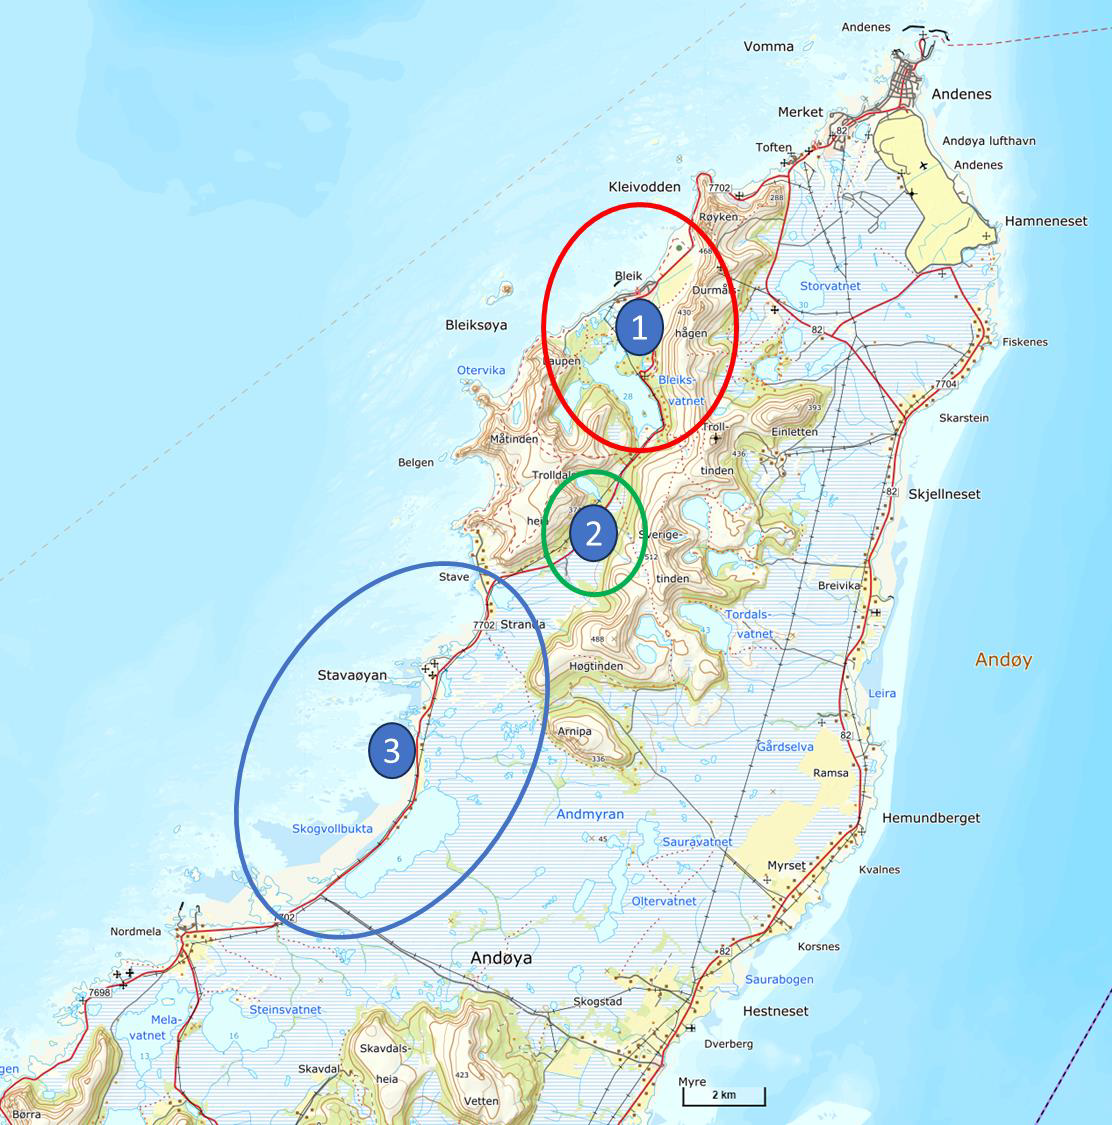
\includegraphics[scale=0.4]{locations.png}

For those wanting more information or have feedback about the test group a technical contact is provided. 

For each test group a set of tests and test varieties are listed with their unique identification number and and name, a text that describes the test. An approximate power number for the transmission. If the test is an automated ramp test then the power range is given. A time estimate of how long the test takes to conclude is given in minutes. Between tests there are also grace periods to allow systems to regain normal operation. These are not given as they are dependent on equipment and needs to be discussed with participants beforehand. The actual grace time will be calculated from the transmission log. The location of the transmitter equipment is also given in the test, this is a coarse human readable description of where the transmitting antenna is located. All participants are encouraged to make their own notes on the location of the transmitting antenna if detailed information is needed. There is also a comment field that can be used to document any other relevant information related to the specific test. 

\chapter{Description of tests}
% Content below is autogenerated 
\section{1: Continuous stationary low power jamming with commercially available jammers}

\subsection*{Rationale}

The main objective is to observe how the J/S signal affect the availability of PNT, and/or how it produces inaccurate PNT data, when the jamming signal (J) is generated by low-power jammers commercially available online. It will also allow participants to create a reference against other, more sophisticated transmission test cases. Additionally, as these types of jammers are the ones one is most likely to meet in the real world, capturing and storing the signals from these jammers for later use in labs could be useful. The use of continuous low power jamming will block out only a certain area. The attendees may therefore test the range of such a low-power jammer. Technical information on jammers can be found as appendix. The jammers used are acquirable from the internet, and each will either be representable for a specific jammer category, or be of special interest for the rest of the test week.

\subsection*{Test setup}

All tests will be performed as follows: The jammer will be activated while placed outside, on top of a stationary vehicle. The jammer will be kept turned on for two (2) minutes, and a two-minute break will be held between each test case. This scenario can be performed and/or repeated at multiple test areas. When activated, all jammers will have all possible GNSS jamming bands activate. If all 28 low effect jammers are tested in sequence, the test will take approximately 2 hours and 2 minutes, which include a 10-minute extra break at the end of the last jammer.

\subsubsection*{Areas}

[ 1 , 3 ]

\subsubsection*{Technical contact}

Nicolai Gerrard, Nkom

\section*{Test within this testgroup}

\subsection{1.1  Jammer S1.1}

\noindent\rule[0.5ex]{\linewidth}{1pt} 
Test with jammer S1.1
\subsubsection*{Power or power range}
1w
\subsubsection*{Test running time}
2 minutes
\subsubsection*{Location of transmitter}
Bleik community parkinglot
\subsubsection*{Comment}
Spesification of jammer can be found list of jammers
\subsection{1.2  Jammer S1.2}

\noindent\rule[0.5ex]{\linewidth}{1pt} 
Test with jammer S1.1
\subsubsection*{Power or power range}
1w
\subsubsection*{Test running time}
2 minutes
\subsubsection*{Location of transmitter}
Bleik community parkinglot
\subsubsection*{Comment}
Spesification of jammer can be found list of jammers

\end{document}

